%!TEX root = ..//Avali-Arena-Esportivas.tex
\section{ AMOSTRA }

\hspace*{1.25 cm} A amostra adotada neste estudo, conforme citado anteriormente, é composta 16 estádios ou arenas esportivas, os quais serão descritos de forma suscinta a seguir. 

\subsection{ ARENA DO GRÊMIO }

%
\hspace*{1.25 cm} O novo estádio do Grêmio foi apresentado pela primeira vez em 2009 como um projeto conceituai pela Plarq Arquitetura, de São Paulo. A construção - financiada com recursos privados do clube - começou em setembro de 2010 e terminou pouco mais de 2 anos depois, em novembro de 2012. Tanto o prazo quanto o orçamento de R\$ 540 milhões não foram excedidos, tornando o estádio exemplar no Brasil.\\ 
%
\hspace*{1.25 cm} A arena, coberta quase inteiramente com elementos azuis, brancos e pretos do escudo do clube, tem capacidade para 60.540 pessoas, com uma arquibancada dedicada aos torcedores da comunidade "Geral" que preferiram não ter assentos. Após adaptações especiais, a arquibancada conseguiu suportar a queda da torcida -comportamento típico da torcida gremista após um gol.\\
\begin{minipage}[t!]{0.5\textwidth}
	\begin{figure}[H]
		\centering  \small 	\caption{ Fotografia externa do Estádio do Grêmio}
		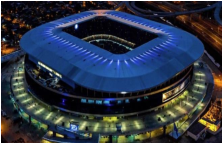
\includegraphics[width=0.69347\linewidth]{figura/screenshot002}
		\label{fig:screenshot002}\\{ Fonte:   http://stadiumdb.com}
	\end{figure}
\end{minipage}\hfill
\begin{minipage}[t!]{0.5\textwidth}
	\begin{itemize}[itemsep=1pt,parsep=1pt]\vspace{0.00mm} 
		\item 	Dados retirados de http://stadiumdb.com \item  Capacidade - 60.540 \item  Construção - 09.2010 -12.2012 \item  Custo - 540 milhões de R\$
	\end{itemize}
\end{minipage} 




\subsection{ALLIANZ PARQUE}
%
\hspace*{1.25 cm} A reconstrução completa de um dos estádios mais bem localizados de São Paulo foi iniciada em 2010, em linha com os preparativos para a Copa do Mundo de 2014. Mas o projeto tinha pouco a ver com o megaevento - era um empreendimento privado do Palmeiras, da WTorre (construtora) e da AEG (maior operadora de entretenimento do mundo). A AEG ganhou acesso ao lucrativo mercado de eventos de São Paulo com este local.\\ 
%
\hspace*{1.25 cm} Desde o início, planejou-se deixar a curva norte da bacia do antigo estádio e incorporá-la ao novo layout. Dessa forma, uma extremidade seria quase retangular, enquanto a outra, oval. O primeiro conceito foi desenhado por Tomas Taveira, enquanto o projeto final ficou a cargo da equipe de Edo Rocha. De acordo com a visão, o revestimento externo consiste em malha metálica perfurada entrelaçada através de estruturas de suporte. O edifício é dominado por cinco torres, que constituem as principais vias de acesso para os torcedores e, ao mesmo tempo, fornecem suporte para a cobertura.\\
\begin{minipage}[t!]{0.5\textwidth}
	\begin{figure}[H]
		\centering  \small 		\caption{Fotografia externa do Estádio Allianz Parque}
		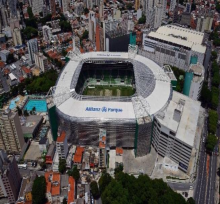
\includegraphics[width=0.69347\linewidth]{figura/screenshot003}
		\label{fig:screenshot003}\\{ Fonte:   http://stadiumdb.com}
	\end{figure}
\end{minipage}\hfill
\begin{minipage}[t!]{0.5\textwidth}
	\begin{itemize}[itemsep=1pt,parsep=1pt]\vspace{0.00mm} 
		\item  Dados retirados de http://stadiumdb.com \item Capacidade - 43.713 \item Construção - 2010 -11/2014 \item Custo - 630 milhões de R\$
	\end{itemize}
\end{minipage} 




\subsection{ESTÁDIO MILTON SANTOS}

\begin{minipage}[t!]{0.5\textwidth}
	\begin{figure}[H]
		\centering  \small 		\caption{Fotografia externa do Estádio Milton Santos}
		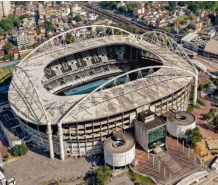
\includegraphics[width=0.6347\linewidth]{figura/screenshot004}
		\label{fig:screenshot004}\\{ Fonte:   http://stadiumdb.com}
	\end{figure}
\end{minipage}\hfill
\begin{minipage}[t!]{0.5\textwidth}
	\begin{itemize}[itemsep=1pt,parsep=1pt]\vspace{0.00mm} 
		\item   Dados retirados de http://stadiumdb.com \item  Capacidade - 44 661 \item  Renovações - 2013, 2016, 2017 \item Custo - 380 milhões de R\$
	\end{itemize}
	
\end{minipage} 




\subsection{ESTÁDIO MARACANÃ}
%
\hspace*{1.25 cm} O Estádio Jornalista Mário Filho, mais conhecido como Maracanã, é um estádio de futebol localizado na Zona Norte da cidade brasileira do Rio de Janeiro. Foi inaugurado em 1950, inicialmente com o nome de Estádio Municipal, durante o mandato do então general de divisão e prefeito do Distrito Federal do Rio de Janeiro Ângelo Mendes de Moraes, tendo sido utilizado na Copa do Mundo de Futebol daquele ano. Quando da sua inauguração, a capacidade oficial de 155 mil lugares fez o Maracanã superar o Hampden Park, de Glasgow, e se tornar o maior estádio do mundo na época.\\ 
%
\hspace*{1.25 cm} Após diversas obras de modernização, a capacidade do estádio é de 78 838 espectadores, sendo o maior estádio do Brasil\\
\begin{minipage}[t!]{0.5\textwidth}
	\begin{figure}[H]
		\centering  \small 	\caption{ Fotografia externa do Estádio Maracanã}
		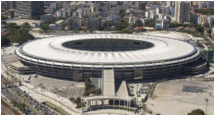
\includegraphics[width=0.69347\linewidth]{figura/screenshot005}
		\label{fig:screenshot005}\\{ Fonte:   http://stadiumdb.com}
	\end{figure}
\end{minipage}\hfill
\begin{minipage}[t!]{0.5\textwidth}
	\begin{itemize}[itemsep=1pt,parsep=1pt]\vspace{0.00mm} 
		\item Dados retirados de http://stadiumdb.com \item Capacidade - 78 838 \item Renovações - 2010-2013 \item Custo -1,14 bilhão de R\$ 
	\end{itemize}	
\end{minipage} 



\subsection{ARENA PANTANAL}
%
\hspace*{1.25 cm} O projeto na zona oeste de Cuiabá foi lançado na primavera de 2010, quando começou a demolição do antigo Verdão. A previsão inicial era de que a obra fosse entregue já em 2012, bem antes da Copa do Mundo de 2014, para a qual o estádio foi encomendado. No entanto, atrasos nas entregas, acidentes e impasses nos pagamentos levaram a atrasos imensos. De fato, o estádio não foi totalmente concluído a tempo para o evento da FIFA de 2014, apesar dos esforços de 1.800 operários no local.\\
\begin{minipage}[t!]{0.5\textwidth}
	\begin{figure}[H]
		\centering  \small 	\caption{ Fotografia externa da Arena Pantanal}
		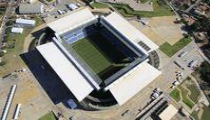
\includegraphics[width=0.69347\linewidth]{figura/screenshot006}
		\label{fig:screenshot006}\\{ Fonte:   http://stadiumdb.com}
	\end{figure}
	
\end{minipage}\hfill
\begin{minipage}[t!]{0.5\textwidth}
	\begin{itemize}[itemsep=1pt,parsep=1pt]\vspace{0.00mm} 
		\item  Dados retirados de http://stadiumdb.com \item Capacidade - 41.930 \item Renovações - 2014 \item Custo - 646 milhões de R\$
	\end{itemize}
	
\end{minipage} 



\subsection{ARENA AMAZONIA}
%
\hspace*{1.25 cm} O estádio está localizado no local do Estádio Vivaldo Lima (comumente chamado de Vivaldão), o antigo maior estádio de Manaus. Embora sua capacidade oficial no fechamento fosse de 31.000 pessoas, o público recorde foi de quase 60.000 pessoas.\\ 
%
\hspace*{1.25 cm} O novo estádio foi batizado de Arena da Amazônia para criar uma referência direta à sua localização e identidade. Seguindo o conceito da GMP Architekten, a estrutura externa do estádio foi projetada para se assemelhar a uma cesta típica da Amazônia, que frequentemente apresenta padrões diagonais. Os assentos do estádio criam um mosaico amarelo-alaranjado que lembra as frutas carregadas na cesta.\\
\begin{minipage}[t!]{0.5\textwidth}
	\begin{figure}[H]
		\centering  \small 		\caption{Fotografia externa da Arena Amazonia}
		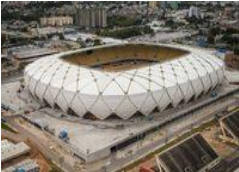
\includegraphics[width=0.69347\linewidth]{figura/screenshot007}
		\label{fig:screenshot007}\\{ Fonte:   http://stadiumdb.com}
	\end{figure}
\end{minipage}\hfill
\begin{minipage}[t!]{0.5\textwidth}
	\begin{itemize}[itemsep=1pt,parsep=1pt]\vspace{0.00mm} 
		\item Dados retirados de http://stadiumdb.com
		\item Capacidade - 44.351
		\item Renovações - 2014
		\item Custo - 669,5 milhões de R\$ 
	\end{itemize}
\end{minipage} 





\subsection{ARENA DAS DUNAS}
%
\hspace*{1.25 cm} As primeiras imagens do estádio foram apresentadas em 2010. Naquela época, a Populous Architects estava no projeto, mas o projeto detalhado foi executado por equipes brasileiras. O estádio, com sua estrutura externa leve e sulcada, tem como característica marcante as escadas expostas, em vez de escondidas sob as arquibancadas.\\
\begin{minipage}[t!]{0.5\textwidth}
	\begin{figure}[H]
		\centering  \small 		\caption{Fotografia externa da Arena das Dunas}
		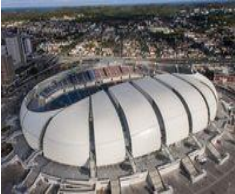
\includegraphics[width=0.69347\linewidth]{figura/screenshot008}
		\label{fig:screenshot008}\\{ Fonte:   http://stadiumdb.com}
	\end{figure}
\end{minipage}\hfill
\begin{minipage}[t!]{0.5\textwidth}
	\begin{itemize}[itemsep=1pt,parsep=1pt]\vspace{0.00mm} 
		\item  Dados retirados de http://stadiumdb.com \item Capacidade - 31.375 \item Inauguração - 2014 \item Custo - 423 milhões de R\$ 
	\end{itemize}
\end{minipage} 





\subsection{ESTÁDIO BEIRA RIO}

%
\hspace*{1.25 cm} A construção do estádio às margens do Rio 1959. As obras foram financiadas por diversas fontes, da torcida do Internacional. Uma das futuras lendas de Porto Alegre foi iniciada em também graças ao engajamento do futebol, Falcão, estava entre os trabalhadores voluntários, então ainda muito jovem.\\
\begin{minipage}[t!]{0.5\textwidth}
	\begin{figure}[H]
		\centering  \small 		\caption{Fotografia externa do Estádio Beira Rio}
		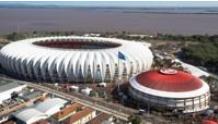
\includegraphics[width=0.69347\linewidth]{figura/screenshot009}
		\label{fig:screenshot009}\\{ Fonte:   http://stadiumdb.com}
	\end{figure}
\end{minipage}\hfill
\begin{minipage}[t!]{0.5\textwidth}
	\begin{itemize}[itemsep=1pt,parsep=1pt]\vspace{0.00mm} 
		\item Dados retirados de http://stadiumdb.com \item Capacidade - 51.800 \item Renovações - 2014 \item Custo - 330 milhões de R\$
	\end{itemize}
	
\end{minipage} 





\subsection{ESTÁDIO PEDRO LUDOVICO TEIXEIRA}
%
\hspace*{1.25 cm} Inicialmente, o estádio estava localizado ao norte do centro, mas, com o tempo, foi se integrando à malha urbana e hoje é o estádio de futebol mais central de Goiânia. Manteve sua forma original até 2006 e foi totalmente demolido posteriormente. A construção do sucessor seria realizada em breve, e a escavação para o novo estacionamento subterrâneo foi feita com antecedência.\\ 
%
\hspace*{1.25 cm} O novo estádio mantém suas funções "olímpicas", oferecendo um campo de jogos e uma pista de atletismo com 8 raias. Com holofotes adicionais, atende à maioria dos critérios nacionais e internacionais. Mesmo após a reconstrução completa, voltou a ser basicamente um estádio de futebol.\\ 
\begin{minipage}[t!]{0.5\textwidth}
	\begin{figure}[H]
		\centering  \small 		\caption{Fotografia externa do Estádio Pedro Ludovico Teixeira}
		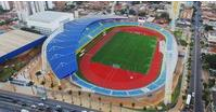
\includegraphics[width=0.69347\linewidth]{figura/screenshot010}
		\label{fig:screenshot010}\\{ Fonte:   http://stadiumdb.com}
	\end{figure}
	
\end{minipage}\hfill
\begin{minipage}[t!]{0.5\textwidth}
	\begin{itemize}[itemsep=1pt,parsep=1pt]\vspace{0.00mm} 
		\item Dados retirados de http://stadiumdb.com \item  Capacidade - 13.500 \item Inauguração - 2016 \item Custo - 96 milhões de R\$ 
	\end{itemize}
\end{minipage} 



\subsection{ESTÁDIO CASTELÃO}
%
\hspace*{1.25 cm} Com o Brasil sendo anunciado como sede da Copa do Mundo de 2014 , outra grande reforma ocorreu em 2011. Desta vez, a arquibancada superior foi mantida, enquanto as arquibancadas inferiores foram reconstruídas, mais próximas do campo e com mais assentos. Apenas a arquibancada principal foi construída completamente do zero, para oferecer instalações para escritórios e serviços de hospitalidade. As obras levaram ao aumento da capacidade, proporcionando também cobertura para todos os espectadores pela primeira vez na história do estádio.\\
\begin{minipage}[t!]{0.5\textwidth}
	\begin{figure}[H]
		\centering  \small 		\caption{Fotografia externa do Estádio Castelão}
		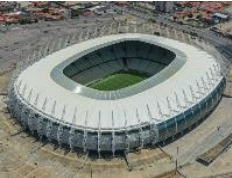
\includegraphics[width=0.69347\linewidth]{figura/screenshot011}
		\label{fig:screenshot011}\\{ Fonte:   http://stadiumdb.com}
	\end{figure}
\end{minipage}\hfill
\begin{minipage}[t!]{0.5\textwidth}
	\begin{itemize}[itemsep=1pt,parsep=1pt]\vspace{0.00mm} 
		\item Dados retirados de http://stadiumdb.com \item Capacidade - 63.903 \item Construção - 2011 / 2013 \item Custo - 518,6 milhões de R\$
	\end{itemize}
	
\end{minipage} 


\subsection{ARENA PERNANBUCO}
%
\hspace*{1.25 cm} As obras nos arredores do Recife começaram em agosto de 2010 e a entrega do novo estádio com muito atraso (nem duas semanas antes da Copa das Confederações de 2013) não é o único resultado do projeto.\\ 
%
\hspace*{1.25 cm} Em maio de 2013, foi assinado um contrato de naming rights de 10 anos com a Itaipava, marca brasileira de cerveja. No valor de cerca de R\$ 100 milhões, o contrato é idêntico ao assinado em Salvador da Bahia e torna o novo estádio pernambucano uma das duas Arenas Itaipava no Brasil.\\
\begin{minipage}[t!]{0.5\textwidth}
	\begin{figure}[H]
		\centering  \small 		\caption{Fotografia externa da Arena Pernambuco}
		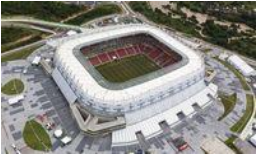
\includegraphics[width=0.69347\linewidth]{figura/screenshot012}
		\label{fig:screenshot012}\\{ Fonte:   http://stadiumdb.com}
	\end{figure}
\end{minipage}\hfill
\begin{minipage}[t!]{0.5\textwidth}
	\begin{itemize}[itemsep=1pt,parsep=1pt]\vspace{0.00mm} 
		\item Dados retirados de http://stadiumdb.com \item Capacidade - 46154 \item Inauguração - 2013 \item Custo - 650 milhões de R\$
	\end{itemize} 
	
\end{minipage} 



\subsection{ARENA MRV}
%
\hspace*{1.25 cm} O projeto para o novo estádio do Atlético Mineiro foi elaborado em 2014, quando o arquiteto Bernardo Farkasvolgyi (torcedor particular do Galo) elaborou o projeto. Um terreno foi adquirido com sucesso da MRV Engenharia, patrocinadora do clube e maior incorporadora do Brasil, com sede em Belo Horizonte, para a construção da arena. Posteriormente, a empresa também adquiriu os direitos de naming do estádio.\\
\begin{minipage}[t!]{0.5\textwidth}
	\begin{figure}[H]
		\centering  \small 	\caption{Fotografia externa da Arena MRV}
		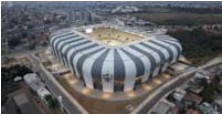
\includegraphics[width=0.69347\linewidth]{figura/screenshot013}
		\label{fig:screenshot013}\\{ Fonte:   http://stadiumdb.com}
	\end{figure}
\end{minipage}\hfill
\begin{minipage}[t!]{0.5\textwidth}
	\begin{itemize}[itemsep=1pt,parsep=1pt]\vspace{0.00mm} 
		\item  Dados retirados de http://stadiumdb.com \item Capacidade - 47.465 \item  Inauguração - 2022 \item Custo - 560 milhões de R\$
	\end{itemize}
\end{minipage} 


%


\subsection{ARENA DO ESPORTE}
%
\hspace*{1.25 cm} Este projeto privado foi alvo de lobby em 2011, mas só tomou forma final com a revelação do projeto da Pontual Arquitetos e Tomas Taveira. O segundo nome deve soar familiar, já que a arena proposta se assemelha a muitos de seus trabalhos anteriores, talvez até demais.\\ 
%
\hspace*{1.25 cm} Sob o revestimento colorido do clube, encontram-se arquibancadas de dois níveis, divididas por três níveis de camarotes comerciais. A capacidade total prevista é de cerca de 46.000 pessoas.\\
\begin{minipage}[t!]{0.5\textwidth}
	\begin{figure}[H]
		\centering  \small 		\caption{Fotografia externa da Arena do Esporte}
		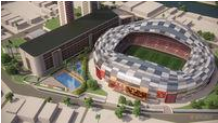
\includegraphics[width=0.69347\linewidth]{figura/screenshot014}
		\label{fig:screenshot014}\\{ Fonte:   http://stadiumdb.com}
	\end{figure}
\end{minipage}\hfill
\begin{minipage}[t!]{0.5\textwidth}
	\begin{itemize}[itemsep=1pt,parsep=1pt]\vspace{0.00mm} 
		\item Dados retirados de http://stadiumdb.com \item Capacidade - 46.000 \item Inauguração - 2016 \item Custo - 600 milhões de R\$
	\end{itemize}
\end{minipage} 




\subsection{ESTÁDIO URBANO CALDEIRA}
%
\hspace*{1.25 cm} Todo o estádio seria envolto em malha de fibra de carbono branca, garantindo ventilação natural. Isso é necessário principalmente porque a cobertura será uma cúpula completa. Em grande parte opaca, a cobertura terá um óculo significativo para fornecer luz natural, com uma tela panorâmica gigante abaixo.\\ 
%
\hspace*{1.25 cm} Atrasos no projeto e custos exorbitantes levaram a mudanças no projeto. Uma das interferências mais visíveis foi o abandono da cobertura total do estádio. Por outro lado, a capacidade das arquibancadas foi aumentada de mais de 25.000 para mais de 30.000 espectadores.\\
\begin{minipage}[t!]{0.5\textwidth}
	\begin{figure}[H]
		\centering  \small 		\caption{Fotografia externa do Estádio Urbano Caldeira}
		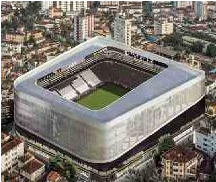
\includegraphics[width=0.69347\linewidth]{figura/screenshot015}
		\label{fig:screenshot015}\\{ Fonte:   http://stadiumdb.com}
	\end{figure}
\end{minipage}\hfill
\begin{minipage}[t!]{0.5\textwidth}
	\begin{itemize}[itemsep=1pt,parsep=1pt]\vspace{0.00mm} 
		\item Dados retirados de http://stadiumdb.com \item Capacidade - 30.108 \item  Inauguração - 2027 \item Custo - 450 milhões de R\$
	\end{itemize}
\end{minipage} 





\subsection{ESTÁDIO INDEPENDÊNCIA}
%
\hspace*{1.25 cm} A demolição do antigo terreno estava planejada para 2008. O América FC recusou o arrendamento do estádio e as obras estavam programadas para começar em 2009. Minas Gerais e o governo federal dividiram o custo entre si, estimado em R\$ 44 milhões. As obras começaram com um atraso de um ano - demolição em janeiro de 2010 e construção de novas arquibancadas em novembro daquele ano. Enormes problemas surgiram ao longo do caminho, com o custo subindo dos primeiros R\$ 44 milhões para 70, 90, 114 e finalmente R\$ 125 milhões.\\
\begin{minipage}[t!]{0.5\textwidth}
	\begin{figure}[H]
		\centering  \small 		\caption{ Fotografia externa do Estádio Independência}
		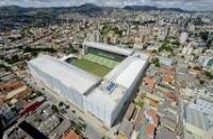
\includegraphics[width=0.69347\linewidth]{figura/screenshot017}
		\label{fig:screenshot017}\\{ Fonte:   http://stadiumdb.com}
	\end{figure}
\end{minipage}\hfill
\begin{minipage}[t!]{0.5\textwidth}
	\begin{itemize}[itemsep=1pt,parsep=1pt]\vspace{0.00mm} 
		\item   Dados retirados de http://stadiumdb.com \item  Capacidade - 23.950 \item Inauguração - 2013 \item Custo - 360 milhões de R\$
	\end{itemize}
\end{minipage} 


\subsection{ARENA DA BAIXADA}
%
\hspace*{1.25 cm} O estádio existente no centro de Curitiba estava programado para ser expandido antes da Copa do Mundo de 2014. Como uma das reformas privadas em todo o Brasil, o objetivo era maximizar os lucros como uma arena multieventos com teto retrátil. No entanto, os painéis móveis foram cortados do plano original devido aos crescentes atrasos.\\ 
%
\hspace*{1.25 cm} O estádio terá um novo lado sul, nova estrutura de cobertura baseada em treliças de aço e uma nova identidade visual.\\
\begin{minipage}[t!]{0.5\textwidth}
	\begin{figure}[H]
		\centering  \small 	\caption{Fotografia externa da Arena da Baixada}
		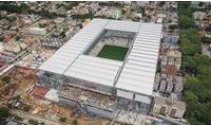
\includegraphics[width=0.69347\linewidth]{figura/screenshot016}
		\label{fig:screenshot016}\\{ Fonte:   http://stadiumdb.com}
	\end{figure}
\end{minipage}\hfill
\begin{minipage}[t!]{0.5\textwidth}
	\begin{itemize}[itemsep=1pt,parsep=1pt]\vspace{0.00mm} 
		\item Dados retirados de http://stadiumdb.com \item Capacidade - 41.375 \item Inauguração - 2012 \item Custo - 360 milhões de R\$
	\end{itemize}
\end{minipage} 

